% Physics and Engineering

\documentclass[11pt]{article}

\usepackage[a4paper, margin=1in]{geometry}

\usepackage{amsmath}

\usepackage{amssymb}

\usepackage[german]{babel}

\usepackage[autostyle=true]{csquotes}

\usepackage{libertine}

\usepackage[libertine]{newtxmath}

\usepackage{tikz}

\usepackage{gensymb}

\usepackage{fancyhdr}

\usepackage{amsfonts}

\usepackage{pgfplots}

\pgfplotsset{compat=1.10}

\usepackage{multicol}

\usepackage{caption}

\usepackage{floatrow}

\everymath{\displaystyle}

% Header / footer settings

\pagestyle{fancy}
\fancyhf{}
\renewcommand{\headrulewidth}{0.2mm}
\fancyhead[C]{Funktionen}
\renewcommand{\footrulewidth}{0.2mm}
\fancyfoot[L]{Peter Goldsborough}
\fancyfoot[C]{\thepage}
\fancyfoot[R]{\today}

\fancypagestyle{plain}{%
	\fancyhf{}
	\renewcommand{\headrulewidth}{0mm}%
	\renewcommand{\footrulewidth}{0.2mm}%
	\fancyfoot[L]{Peter Goldsborough}
	\fancyfoot[C]{\thepage}
	\fancyfoot[R]{\today}
}


\setlength{\headheight}{15pt}

\setlength{\parindent}{0pt}

\addtolength{\parskip}{\baselineskip}


\newcommand{\overbar}[1]{\mkern 1.5mu\overline{\mkern-1.5mu#1\mkern-1.5mu}\mkern 1.5mu}

\newcommand{\heading}[1]{\begin{center}\Huge \textbf{#1}\end{center}\par}

\newcommand{\sub}[1]{\vspace{\parskip}{\LARGE\textbf{#1}}}

\newcommand{\subsub}[1]{{\Large \textbf{#1}}}

\newcommand{\subsubsub}[1]{\textbf{#1}}

\newcommand{\colvec}[1]{\begin{pmatrix}#1\end{pmatrix}}

\newcommand{\extrapar}{\par\vspace{\baselineskip}}

\newcommand{\zitat}[1]{\foreignquote{german}{#1}}

\newcommand{\bolditem}[1]{\item \textbf{#1}}

\newcommand{\titleitem}[1]{\bolditem{#1}\par}

\newcommand{\defas}{ \dots \,\,}

\begin{document}
\thispagestyle{plain}

\heading{Physics and Engineering}

\sub{Transformers}

A transformer is a device for changing an alternating voltage from one value to another. It plays a significant role in the distribution and use of electric power for industry and in everyday life. Transformers \emph{step-up} (increase) the voltage produced by an AC generator to very high values to ensure efficient transmission across large distances.  Subsequently, substations near to households \emph{step-down} (decrease) the voltage to 230 Volts or other standard values which depend on the particular country. In homes, small transformers in phone or laptop chargers or other electrical devices step-down the voltage further to values that are safe and appropriate for them, often 9 Volts. The underlying principles of such a transformer are those of electromagnetism and electromagnetic induction. 

\subsub{Setup and Working Principle}

The basic construction and configuration of a transformer involves two conductive coils of wire wrapped around a closed loop of a soft iron core. One of the two coils is referred to as the \emph{primary coil}, situated on the \emph{primary side} of the transformer. The second coil, on the other end of the soft iron core --- the \emph{secondary side}, is called the \emph{secondary coil}. Each coil is characterized by a certain number of windings or turns $N_1$ and $N_2$. When the primary coil is connected to a supply of alternating current with a potential difference $U_1$ across it, an alternating magnetic field is generated around and within the coil. Consequently, the soft iron core is magnetized such that an alternating magnetic flux is present within it. As this changing magnetic flux travels through the closed loop of the soft iron core and reaches the secondary side, it statisfies the requirement for the induction of a potential difference $U_2$ within the secondary coil. This requirement, as per Faradays' law of induction, is that there either be moving conductor in a permanent magnetic field, or, as is the case here, a stationary conductor in an alternating magnetic field. 

\begin{circuit}

	% Primary coil
	\draw (-2, 1.5) -- ++(2, 0)
	      to [cute inductor, l_=$N_1$] ++(0, -1.5) -- ++(-2, 0)
	      to [sinusoidal voltage source, l^=$U_1$] ++(0, 1.5);

	% Soft iron core, outer layer
	\draw [very thick]
	      (-1, -1) -- ++(0, 3.5)
	 -- ++(5, 0) node [midway, above] {Soft Iron Core}
	 -- ++(0, -3.5)
	 -- ++(-5, 0);

	% Soft iron core, inner layer
	\draw [very thick]
	      (0.5, 0) -- ++(0, 1.5)
	 -- ++(2, 0) -- ++(0, -1.5)
	 -- ++(-2, 0);


	% Secondary coil
	\draw (5, 0) -- ++(-2, 0)
	      to [cute inductor, l_=$N_2$] ++(0, 1.5) -- ++(2, 0)
	      to [voltmeter, l^=$U_2$] ++(0, -1.5);

\end{circuit}

The purpose of the soft iron core is to increase the effect of the magnetic field generated as well as to concentrate and guide and the magnetic flux from the primary to the secondary side. Moreover, it reduces magnetic field leakage to a minimum in order to ensure maximum transformer efficiency. However, it should also be mentioned that the conversion and stepping-down or stepping-up of one voltage to another produces not only a magnetic field, but additionally generates thermal energy (heat), which reduces the efficiency of the conversion process. To counteract this, the soft iron core is in fact a sandwich of soft iron plates and insulating material. In such a structure, referred to as \emph{laminated iron}, one layer of soft iron follows one layer of insulation, followed by another layer of soft iron and so on. This ensures maximum possible insulation and efficiency.

\pagebreak

\begin{figure}[h!]
	\centering
	\begin{tikzpicture}

	% Layers
	\foreach \i in {0, 1}
	{
		\draw [fill=gray]
		      (0, \i)
		 -- ++(5, 0) -- ++(0, 0.5) -- ++(-5, 0) -- ++(0, -0.5);

		\draw [fill=red]
		      (0, \i + 0.5)
		 -- ++(5, 0) -- ++(0, 0.5) -- ++(-5, 0) -- ++(0, -0.5);
	}

	% Labels
	\draw [<-] (5.5, 0.25) -- ++(2, 0) node [right] {Soft Iron Core};
	\draw [<-] (5.5, 1.75) -- ++(2, 0) node [right] {Insulation};

	\end{tikzpicture}
	\caption*{The sandwiched layers of the laminated iron core}
\end{figure}

\subsub{Transformer Equations}

In case of a \emph{step-down} transformer, the voltage $U_1$ across the primary coil is greater than the induced voltage $U_2$ across the secondary coil. This can only be the case if the same relationship is true for the turns of the two coils. By contrast, the primary voltage $U_1$ is less than the secondary potential difference $U_2$ when the number of turns of the secondary coil $N_2$ is greater than the number of turns on the primary coil $N_1$. This form of transformer is then referred to as a \emph{step-down} transformer. 

\begin{table}[h!]
	\centering
	\begin{tabular}{l l l}
		
		Step-Up Transformer: & $U_2 > U_1$ & $N_2 > N_1$
		\\ && \\
		Step-Down Transformer: & $U_2 < U_1$ & $N_2 < N_1$

	\end{tabular}
\end{table}

In general, the induced voltage $U_2$ across the secondary coil can be calculated by slightly altering Faraday's law of induction. This law states that the induced potential difference across a conductor in an alternating magnetic field is equal to the negative of the rate of change of magnetic flux. For transformers, there is an extra factor added to this rate of change: the number of turns $N_2$ of the secondary coil. This yields the following expression for the secondary voltage $U_2$: $$U_2 = -N_2 \cdot \frac{d \Phi_m}{d t}$$ However, the alternating magnetic flux does not only effect the secondary coil, but also causes \emph{self-induction} in the primary coil, as the magnetic flux is also changing on the primary side. Therefore, the above definition for the induced voltage $U_2$ on the secondary side can also be used to determine the self-induced voltage $U_{ind}$ across the primary coil. This induced voltage is then equal to the negative of the voltage $U_1$ across the primary coil: $$U_{ind} = -N_1 \cdot \frac{d \Phi_m}{d t} = -U_1 \thus \frac{d \Phi_m}{d t} = \frac{U_1}{N_1}$$ The right side of this equation can then be substituted for the rate of change of magnetic flux in the expression given above for the secondary voltage $U_2$: $$U_2 = -N_2 \cdot \frac{d \Phi_m}{dt} = -N_2 \cdot \frac{U_1}{N_1}$$ This finally yields the following relationship, referred to as the \emph{first transformer law}, where the minus sign indicates a $180\degree$ or $\pi$ radians phase shift between the two voltages $U_1$ and $U_2$, as a result of them being wound in the same direction: $$\frac{U_1}{N_1} = -\frac{U_2}{N_1}$$ Were now a load to be connected on the secondary side (e.g. a lamp), the induced voltage $U_2$ would cause an alternating current $I_2$ to start flowing through the secondary coil. As a result, there would also be an alternating magnetic field generated on the secondary side. This magnetic field would in turn also magnetize the soft iron core, leading to a very complex phase relationship between the magnetic flux created by the primary coil and the magnetic flux created by the scoendary coil. In case of an ideal transformer with 100\% percent efficiency and no loss energy of electrical energy to thermal energy, the total power of the primary coil $P_1$ equals the power of the secondary coil $P_2$. Given that the electrical power of a circuit is equal to the voltage across it multiplied by the current flowing through it, one can determine the following relationship --- known as the \emph{second transformer law} --- between the voltage and current of the two sides of a transformer: $$P_1 = P_2 \thus U_1 \cdot I_1 = U_2 \cdot I_2 \thus \frac{U_1}{U_2} = \frac{I_2}{I_1}$$ One last thing to mention is that in reality, no transformer is really ideal, thus the effective voltage $U_{eff}$ across the primary coil is actually equal to the maximum possible primary voltage $U_{max}$, divided by the square root of two (this can also be used to calculate the maximum voltage given the effective voltage): $$U_{eff} = \frac{U_{max}}{\sqrt{2}}$$

\sub{Power Transmission across the Country}

Unfortunately, no conductor is ideal. There is always some portion of electrical power generated by power stations that is lost during transmission of the power across the country. Especially over great distances the loss in power can be very significant, such that the efficiency is too low for practical use. Thus, great care must be taken to ensure maximum efficiency. One way of doing so is to increase the voltage during transmission. To see why, it must first be discussed how the power $P_{lost}$ can be calculated. In general, electrical power is defined as the voltage across a conductor multiplied by the current flowing through it. Moreover, voltage may be defined not only as a potential difference, but also as the product of current and resistance. This leads to the following equation for the power lost during transmission across the country: $$P_{lost} = U \cdot I = R \cdot I \cdot I = R \cdot I^2$$ The efficiency of transmission may then be calculated as the ratio between the power lost $P_{lost}$ and the power $P$ generated by a given power station (this value could be multiplied by 100 percent to get a direct percentage value for the ratio between the power lost and the power generated): $$\frac{P_{lost}}{P}$$ When expanding both variables, it can be found that the efficiency is equal to the power generated, multiplied by the resistance and divided by the square of the voltage. This shows that it is not necessary to explicitly know the power lost. It can be calculated already from the value of the power generated. $$\frac{P_{lost}}{P} = \frac{R \cdot I^2}{U \cdot I} = \frac{R \cdot I}{U} = \frac{R \cdot I \cdot U}{U \cdot U} = \frac{P \cdot R}{U^2}$$ What this shows is that the power-lost-to-power-generated ratio is inversely proportional to the voltage generated. A greater voltage will thus cause less loss in power. Proof for 20 kilo-volts, 100 kilo-volts and 380 kilo-volts at 1 giga-watts of power transmitted through a conductor with 50 $\Omega$ of resistance are given below.

20 kV: $\frac{P \cdot R}{U^2} = \frac{1 \cdot 10^9 \cdot 50}{(20 \cdot 10^3)^2} \cdot 100\% = 12500 \%$ 

Conclusion: The power lost is 12500 \% of the power generated (none will reach the end user).

\pagebreak

100 kV: $\frac{P \cdot R}{U^2} = \frac{1 \cdot 10^9 \cdot 50}{(100 \cdot 10^3)^2} \cdot 100\% = 500 \%$

Conclusion: Still none.

380 kv: $\frac{P \cdot R}{U^2} = \frac{1 \cdot 10^9 \cdot 50}{(380 \cdot 10^3)^2} \cdot 100\% = 35 \%$ 

Conclusion: Only 35 \% of the power generated is lost, such that it will reach the end user with an efficiency rating of 65 \%.

\sub{Broadcasting}

Broadcasting is the transmission of information --- mostly radio and television signals --- via \emph{radio waves}. Radio waves are found on the lower end of the electromagnetic spectrum, in a frequency range of about $3 \cdot 10^4$ to $3 \cdot 10^9$ Hz. There are three categories into which radio waves are generally divided: \emph{ground} or \emph{surface waves}, \emph{sky waves} and \emph{space waves}. 

\subsub{Ground Waves}

Ground waves (also referred to as surface waves) have the longest wavelength and lowest frequency of the three categories of radio waves, with their frequency typically found at around or below 3 mega-hertz ($3 \cdot 10^6$ Hz). Ground waves are most commonly used for long-distance communication and broadcasting. The reason has to do with the diffraction of waves --- the phenomenon whereby waves are bent when passing through gaps or around obstacles. The degree to which a wave is diffracted depends on its wavelength $\lambda$. In this case, a greater wavelength causes a greater degree of diffraction to occur. As ground waves have the highest wavelength of all radio waves, they are diffracted most as they travel on the surface of the earth, following the curvature of the surface and continuously being bent.

\subsub{Sky Waves}

Sky waves have a higher frequency than ground waves, typically in a range of 3 to 30 mega-hertz ($3 \cdot 10^6 - 3 \cdot 10^7$ Hz), and thus have a shorter wavelength. This also means that they are less suitable for long-distance communication taking place near to the surface of the earth, as a shorter wavelength would cause such a sky wave to experience less diffraction. However, at this frequency the waves do have the ability to propgate through the earth's atmosphere, up to a layer known as the \emph{ionosphere}. The ionosphere is an electrically charged region above the atmosphere, around 50 to 500 kilometers above the surface of the earth, where ultraviolet radiation from the sun results in a high number of positively or negatively charged particles (\emph{ions}) to be found at such altitudes. The intensity of solar radiation and thus ionization changes over time, as the level of radiation from the sun is, of course, less during the night and greater during the day. When sky waves reach the ionosphere, they are \emph{reflected} similar to the way in which light is reflected in the process of total internal reflection. After reflection from the ionosphere, sky waves propagate back to the earth's surface, either to reach their destination directly (\emph{single-hop-transmission}) or to be reflected once more towards the ionosphere after being received by an antenna on the surface of the earth and subsequently re-transmitted. 

\subsub{Space Waves}

Space waves have the highest frequency of all radio waves and thus experience practically no diffraction at all. Therefore, they cannot be used for long-distance near-surface transmission as ground waves can be. Moreover, they are no longer reflected by the ionosphere, but can now pass through it. As a result, space waves are commonly used for satellite communication or direct transmission of signals betwee antennae and in general any form of \emph{line-of-sight-communication}, where the receiving antenna is within the transmitter's line of sight (i.e. a direct, straight path of tranmission) and where diffraction may even be unwanted. This is also a reason why short-wavelength radio waves similar in frequency to space waves are used for the \emph{Bluetooth} protocol between smartphones or other electronic devices such as printers, loudspeakers or computer keyboards. The reason why Bluetooth has only a very short range of usability should now be clear.

\begin{figure}[h!]
	\centering
	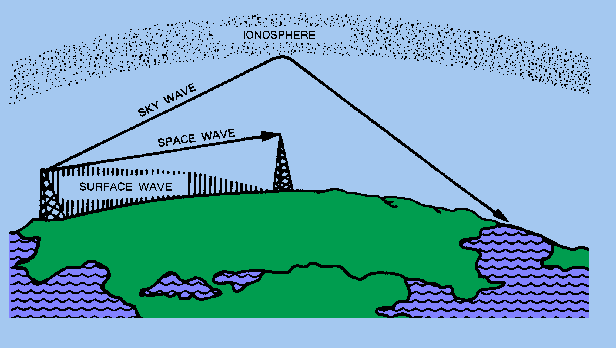
\includegraphics[scale=0.65]{img/radio}
	\caption*{The three categories of radio waves}
\end{figure}


\sub{LC-Circuits}

Electromagnetic waves are transverse waves that travel at the speed of light and consist of a magnetic field and an electric field component, whose field strengths oscillate perpendicular to each other and to the direction of the wave's motion. They find a plethora of applications in everyday life and especially in the transmission of data or signals for television, radio or telecommunications. The most common method of generating such electromagnetic waves is what is known as an \emph{LC-circuit}.

\subsub{Setup of an LC-Circuit}

The configuration or setup of an LC-circuit consists of two main components: a \emph{capacitor} and an \emph{inductor} (a coil). An important property associated with the inductor is its \emph{self-inductance} $L$, measured in henries $[H]$. On the other hand, the capacitor --- an electrical component used to store a certain electrical charge --- is characterized by its capacitance $C$, measured in farads $[F]$. The capacitor and the inductor are connected in a closed series circuit, where also a switch may be present to interrupt the flow of current.

\begin{circuit}
	
	\draw (0, 0)
	      to [cute inductor, l_=$L$] ++(0, -2)
	 -- ++(3, 0)
	      to [capacitor, l_=$C$] ++(0, 2)
	      to [opening switch] ++(-3, 0);

\end{circuit}

\subsub{0. Charging the Capacitor}

Initially, to eventually produce electromagnetic waves, the capacitor must be given a certain electrical charge. For this, the switch is opened and the capacitor is connected to a power supply, which charges the plates of the capacitor. As it does so, one of the plates of the capacitor is charged negatively while the other plate receives a positive charge. Consequently, a homogenous electric field is produced between the positive and the negative plate of the capacitor. The property of homogeneousness refers to the fact that the electric field is equal in strength and density at every point between the two plates.

\begin{circuit}
	
	\draw (0, 0)
	      to [cute inductor, l_=$L$] ++(0, -2)
	 -- ++(5, 0)
	 	  to [battery1] ++(0, 2)
     -- ++(-2, 0) ++(0, -2)
	      to [capacitor, l_=$C$] ++(0, 2)
	      to [opening switch] ++(-3, 0);

	% Charges
	\foreach \i in {-0.1, 0.15, 0.45, 0.7}
	{
		\draw [red] (2.7 + \i, -0.7) node {\footnotesize $+$};

		\draw [blue] (2.7 + \i, -1.3) node {\footnotesize $-$};
	}

	% Field lines
	\foreach \i in {0, 0.2, 0.4, 0.6}
	{
		\draw [->] (2.7 + \i, -0.9) -- ++(0, -0.2);
	}

\end{circuit}

\subsub{1. Closing the Switch}

Next, the battery is removed and the switch is closed. Current then starts to flow and the capacitor gradually discharges. As current flows through the turns of the inductor, a magnetic field is produced within and around it. As this inductor is essentially a coil or solenoid, the shape of the magnetic field generated is similar to that of a bar magnet.  At this stage, the electric field strength $\vec{E}$ decreases with time while, simultaneously, the strength of the magnetic field $\vec{B}$ generated by the current flowing through the inductor is continuously increasing. 

\begin{circuit}
	
	\draw (0, 0)
	      to [cute inductor] ++(0, -2)
	      to [short, i_=$I$] ++(3, 0)
	      to [capacitor] ++(0, 2)
	 	  to [short, i_=$I$] ++(-3, 0);

	% Charges
	\foreach \i in {0, 0.6}
	{
		\draw [red] (2.7 + \i, -0.7) node {\footnotesize $+$};

		\draw [blue] (2.7 + \i, -1.3) node {\footnotesize $-$};
	}

	% Field lines
	\foreach \i in {0.1, 0.5}
	{
		\draw [->] (2.7 + \i, -0.9) -- ++(0, -0.2);
	}

	% Electric field
	\draw [->] (4, -0.5) -- ++(0, -1)
	      node [right, midway] {$\vec{E}$ decreases};

	% Magnetic field
	\draw [<-] (-1, -0.5) -- ++(0, -1)
	      node [left, midway] {$\vec{B}$ increases};


	% Magnetic field lines
	\foreach \a/\b/\c/\d/\e in {0.1/-0.3/0.5/0.3/-1.6,
								0/-0.5/0.3/0.1/-1.4}
	{
		% First side
		\draw [red, ->] (\a, -0.7)
	      .. controls (\d, \b) and (\c, -0.5) .. (\c, -1);

	    \draw [red] 
	          (\c, -1.05) .. controls (\c, -1.5) and (\d, \e) .. (\a, -1.3); 

	    % Second side
		\draw [red, ->] (-\a, -0.7)
	      .. controls (-\d, \b) and (-\c, -0.5) .. (-\c, -1);

	    \draw [red]
	          (-\c, -1.05) .. controls (-\c, -1.5) and (-\d, \e) .. (-\a, -1.3); 
	}

\end{circuit}

\subsub{2. Capacitor discharges}

As the capacitor gradually discharges and is almost entirely void of charges, the magnetic field strength $\vec{B}$ also nears its maximum strength. At one point, the capacitor is then \emph{fully} discharged, such that the current eventually stops flowing. At this point, the magnetic field reaches its maximum and then begins to decrease in strength.

\begin{circuit}
	
	\draw (0, 0)
	      to [cute inductor] ++(0, -2)
	      to [short] ++(3, 0)
	      to [capacitor] ++(0, 2)
	 	  to [short] ++(-3, 0);

	% Electric field
	\draw (4, -1) node [right] {$\vec{E}$ at minimum};

	% Magnetic field
	\draw (-1, -1) node [left] {$\vec{B}$ at maximum};


	% Magnetic field lines
	\foreach \a/\b/\c/\d/\e in {0.1/-0.3/0.5/0.3/-1.6,
								0/-0.5/0.3/0.1/-1.4,
							    0/-0.1/0.7/0.4/-1.6}
	{
		% First side
		\draw [red, ->] (\a, -0.7)
	      .. controls (\d, \b) and (\c, -0.5) .. (\c, -1);

	    \draw [red] (\c, -1.05) .. controls (\c, -1.5) and (\d, \e) .. (\a, -1.3); 

	    % Second side
		\draw [red, ->] (-\a, -0.7)
	      .. controls (-\d, \b) and (-\c, -0.5) .. (-\c, -1);

	    \draw [red] (-\c, -1.05) .. controls (-\c, -1.5) and (-\d, \e) .. (-\a, -1.3); 
	}

\end{circuit}

\subsub{3. Induction of Current}

This decrease in the magnetic field strength signifies a change in the magnetic flux in the coil, leading it to \emph{self-induce} a voltage and consequently a current. The direction of the induced current $I_{ind}$ is the same as that of the original current $I$. The reason for this can be derived from Lenz' law, which states that:

\begin{displayquote}

	The direction of the induced voltage is such that, were an induced current able to flow, it would oppose the change that caused it.

\end{displayquote}

The change that caused the induction of the the current was the \emph{breaking-down} of the magnetic field of the inductor. As stated by Lenz law, the induced current always flows in the direction that acts against the change that caused it. It thus must try to keep the magnetic field constant and stop its degeneration. The only way for it to do so is to keep flowing in the same direction, as this is the direction that caused the field to increase initially. The side-effect of this is the most important property of the LC-circuit: the capacitor is gradually re-charged in the opposite way --- with opposite polarity. 

\begin{circuit}
	
	\draw (0, 0)
	      to [cute inductor] ++(0, -2)
	      to [short, i_=$I_{ind}$] ++(3, 0)
	      to [capacitor] ++(0, 2)
	 	  to [short] ++(-3, 0);

	% Charges
	\foreach \i in {0, 0.6}
	{
		\draw [blue] (2.7 + \i, -0.7) node {\footnotesize $-$};

		\draw [red] (2.7 + \i, -1.3) node {\footnotesize $+$};
	}

	% Field lines
	\foreach \i in {0.1, 0.5}
	{
		\draw [<-] (2.7 + \i, -0.9) -- ++(0, -0.2);
	}

	% Electric field
	\draw [<-] (4, -0.5) -- ++(0, -1)
	      node [right, midway] {$\vec{E}$ increasing};

	% Magnetic field
	\draw [->] (-1, -0.5) -- ++(0, -1)
	      node [left, midway] {$\vec{B}$ decreasing};

	% Magnetic field lines
	\foreach \a/\b/\c/\d/\e in {0.1/-0.3/0.5/0.3/-1.6,
								0/-0.5/0.3/0.1/-1.4}
	{
		% First side
		\draw [red, ->] (\a, -0.7)
	      .. controls (\d, \b) and (\c, -0.5) .. (\c, -1);

	    \draw [red] 
	          (\c, -1.05) .. controls (\c, -1.5) and (\d, \e) .. (\a, -1.3); 

	    % Second side
		\draw [red, ->] (-\a, -0.7)
	      .. controls (-\d, \b) and (-\c, -0.5) .. (-\c, -1);

	    \draw [red]
	          (-\c, -1.05) .. controls (-\c, -1.5) and (-\d, \e) .. (-\a, -1.3); 
	}

\end{circuit}

\subsub{4. Capacitor fully re-charged}

At last, the capacitor is again fully charged, such that the electric field $\vec{E}$ is again at its maximum, while the magnetic field $\vec{B}$ is no longer present at all, such that $|\vec{B}| = 0$. 

\begin{circuit}
	
	\draw (0, 0)
	      to [cute inductor] ++(0, -2)
	      to [short] ++(3, 0)
	      to [capacitor] ++(0, 2)
	 	  to [short] ++(-3, 0);

	% Charges
	\foreach \i in {-0.1, 0.15, 0.45, 0.7}
	{
		\draw [blue] (2.7 + \i, -0.7) node {\footnotesize $-$};

		\draw [red] (2.7 + \i, -1.3) node {\footnotesize $+$};
	}

	% Field lines
	\foreach \i in {0, 0.2, 0.4, 0.6}
	{
		\draw [<-] (2.7 + \i, -0.9) -- ++(0, -0.2);
	}

	% Electric field
	\draw (4, -1) node [right] {$\vec{E}$ at maximum};

	% Magnetic field
	\draw (-1, -1) node [left] {No $\vec{B}$};

\end{circuit}

The whole cycle would repeat once more, just that the polarity of the capacitor is now reversed. After the next half-cycle, the polarity would again match its original configuration. If energy losses are neglected, this oscillatory behaviour could go on ad infinitum. In conclusion, it can be said that, for an LC-circuit \dots

\begin{itemize}
	
	\item \dots the charges oscillate between the plates of the capacitor

	\item \dots the energy oscillates between the electric field $\vec{E}$ and the magnetic field $\vec{B}$

	\item \dots the field strengths of both the electric field $\vec{E}$ and the magnetic field $\vec{B}$ oscillate

\end{itemize}

The frequency with which this oscillation takes place can be determined using an equation referred to as the \emph{Thomson formula}. Its derivation is fairly simple, if it is known that the angular frequency $\omega$ of the charge and energy oscillation is equal to the inverse square root of the product of the self-inductance $L$ of the coil and the capacitance $C$ of the capacitor. Moreover, it must be remembered that the angular frequency $\omega$ of any object or system undergoing periodic behaviour is equal to two $\pi$ times the frequency $f$. Thus, the frequency $f$ must be equal to $\omega$ divided by $2 \pi$. $$\omega = \frac{1}{\sqrt{L \cdot C}} \hspace{1cm} \omega = 2\pi \cdot f \Rightarrow f = \frac{\omega}{2\pi}$$ Inserting the angular frequency of an LC-circuit as defined above into the right equation yields the Thomson formula for the determination of the frequency of oscillation of an LC-circuit: $$f = \frac{1}{2\pi} \cdot \frac{1}{\sqrt{L \cdot C}}$$

\pagebreak

\sub{The Hertz Dipole}

It was just shown how an LC-circuit can be used to generate a charge and energy oscillation between a capacitor and an inductor. Moreover, it was stated that the angular frequency $\omega$ of the oscillation is equal to the inverse square root of the self-inductance $L$ multiplied by the capacitance $C$. Taking a closer look at this definition, it can be seen that to increase the angular frequency, one would either have to decrease the self-inductance $L$ of the coil or decrease the capacitance $C$ of the capacitor, or both.

\subsub{Decreasing $L$}

To decrease the self-inductance $L$, one needs to reduce the number of turns of the coil. The minimum number of turns is, of course, one turn. Thus, the inductor is essentially turned into a single loop of wire. Consequently, the field lines of the magnetic field produced are structured in concentric circles around the wire, such that the magnetic field strength $B$ decrases with an increasing distance $r$ from the wire, as per the defintion of the field strength $B$ of the magnetic field generated around a single wire: $$B = \frac{\mu_0}{2 \pi} \cdot \frac{I}{r}$$ Furthermore, it can be observed that the magnetic field is initially very small closer to the positive plate, reaches its maximum in the middle of the wire and finally decrases again as it nears the negative plate (the same could be said for electrons moving in the opposite direction).

\begin{plot}

	\draw (1, 0) arc (20:340:1) % Single loop of the inductor
	      to [capacitor] (1, 0);

	% Charges
	\foreach \i in {0.6, 0.85, 1.15, 1.4}
	{
		\draw [red] (\i, 0) node {\small $+$};

		\draw [blue] (\i, -0.57) node {\small $-$};
	}

	% Field lines
	\foreach \i in {0.7, 0.9, 1.1, 1.3}
	{
		\draw [->] (\i, -0.24) -- ++(0, -0.2);
	}

	% Magnetic field
	\foreach \i in {1, 2, 3, 4}
	{
		\foreach \j in {1, ..., \i}
		{
			\draw [red] (0, -{tan(20)})+({\i * 45}:0.99)
			            circle [radius={0.1 + \j/10}];

			\ifnum\i<4
				\draw [red] (0, -{tan(20)})+({\i * -45}:0.98)
			            circle [radius={0.1 + \j/10}];
			\fi
		}
	}

	% Electric field label
	\draw (1.8, -0.28) node {$\vec{E}$};

\end{plot}

\subsub{Decreasing $C$}

The capacitance $C$ is determined by the distance between the two plates of the capacitor, as well as the size of the plates. Thus, one would first decrease the size of the plates to two single points of the same cross-sectional area as that of the wire. Then, one would entirely open up the single loop of wire and thus LC-circuit, to increase the distance to a maximum. As one does so slowly, one would notice that the electric field between the plates of the capacitor begins to spread out into space. When the loop is then opened up to an entirely straight wire, the LC-circuit can be described by the following properties: 

\begin{itemize}
	
	\item It is a \textbf{straight} wire, but still essentially an inductor coil (with onely one loop, in a very deformed shape)

	\item The plates of the capacitor have been reduced to \textbf{single points}

	\item The electric field and magnetic field are \textbf{no longer separated}. Rather, they \textbf{overlap}.

	\item Both the electric and the magnetic field go \textbf{around the wire}. This was not the case for the electric field before; it used to only be present between the plates of the capacitor.

	\item The \textbf{length} of the wire remains the only variable to change the frequency, as the capacitance depends on the distance between the plates.

\end{itemize}

\pagebreak

\begin{plot}
	
	% Inductor
	\draw [<-]
	      (0, 0, 0) node [below] {$-$}
	   -- (0, 6, 0) node [above] {$+$}
	      node [above, right] {$I$};

	% Electric Field
	\foreach \i in {0.7, 1.2, 1.7}
	{
		\draw [blue] (0, 0) .. controls (\i, 3) .. (0, 6);

		\draw [blue] (0, 0) .. controls (-\i, 3) .. (0, 6);
	}

	% Magnetic Field
	\foreach \y in {1, ..., 5}
	{
		\begin{scope}[canvas is zx plane at y=\y]

		\newcount\n
		\n\y\relax

		\ifnum\n>3
			\advance \n by -6\relax
			\multiply \n by -1\relax
		\fi

		\foreach \r in {1, ..., \n}
		{	
			\draw [<-, red] ({\r * 0.4}, 0) arc (0:350:{\r * 0.4});
		}


		\end{scope}
	}

\end{plot}

\end{document}